% ============================================================
% FOREST FIRE RISK - PROGRESS REPORT (due Sunday 1 November 2026, 23:59)
% Built from the official BAM project template (bam-project.cls v1.2).
%
% While writing:   \documentclass[annotated,onecolumn]{bam-project}
%                  -> grey guidance boxes and placeholders are visible.
% To check length: switch to [clean,onecolumn] and recompile.
%                  Max two pages of text after the cover page;
%                  figures and tables go at the end (sections/98b_figures_tables.tex).
% Before submit:   [clean,onecolumn], every box and placeholder gone.
%
% Each person edits only their own file in sections/.
% Main.tex (metadata, section order, summary) is owned by Claudia.
% Plan: https://claude.ai/artifact/RHxHPnvroeC1p9cxkzmXXE
% ============================================================

% The IE Overleaf server has a minimal TeX Live. These two lines make the
% template work there; on a full TeX Live they change nothing visible.
\def\BAMplainfonts{}                          % skip T1 fonts (not installed)
\makeatletter\def\input@path{{texmf/}}\makeatother  % packages we bundled

\documentclass[clean,onecolumn]{bam-project}

% Numbered bibliography style, as in the template. Cite with \cite{key};
% entries live in references.bib. amsplain.bst is bundled in the project
% root because the IE server lacks it (BibTeX only looks there, not in texmf/).
\BAMbibliographystyle{amsplain}
\BAMbibliographyfile{references}

\graphicspath{{figures/}}

% ============================================================
% PROJECT METADATA
% ============================================================
\BAMtitle{Forest Fire Risk Classification with Multi-Modal Machine Learning: Progress Report}
\BAMshorttitle{Forest Fire Risk: Progress Report}
\BAMcourse{Machine Learning}
\BAMteam{Claudia González\\[0.2em]Sophia Kanashina\\[0.2em]Alexandru Rodideal}
\BAMinstructors{Nacho Molina Clemente}
\BAMsubmissiondate{1 November 2026}

\begin{document}

\makebamtitle
\BAMannotationnotice

% ============================================================
% SUMMARY - Claudia
% ============================================================
\begin{BAMabstract}
\annotation{\textbf{[Owner: Claudia | about 60 words]} Restate the research question (unchanged from the proposal), name the four models (logistic regression, random forest, CNN, fusion), and give the headline result so far with its number. End with the repository and map links.}

For our project, we ask: Does combining Sentinel-2 satellite images with a tabular random forest improve daily wildfire classification over the Mediterranean, and are the two sources complementary or redundant? We trained a logistic regression model, a random forest, a CNN on image tiles, and a fusion model combining the last two on 10,922 samples. On the test years (2021-2022), fusion showed an AUPRC of 0.864, whilst CNN had 0.749 and RF 0.829, showing a clear improvement in fire prediction.


\noindent Code: \url{https://github.com/cgonzalezieu2025-lab/forest-fire-risk}\\
Map: \url{https://forest-fire-risk-map.vercel.app}
\end{BAMabstract}

% ============================================================
% 1. RECAP AND CHANGES SINCE THE PROPOSAL - Claudia (~150 words)
% ============================================================
\section{Recap and Changes Since the Proposal}
\label{sec:recap}

\annotation{\textbf{[Owner: Claudia | about 150 words]} Remind the reader of the question in one sentence, describe the final sample set once (the other sections refer back here instead of repeating it), and justify every change from the proposal. The brief asks us to ``justify the choices made''.}

\annotation{\textbf{[Cover]}
(1) Research question, one sentence: does fusing a Sentinel-2 CNN with a tabular random forest beat either source alone, and are the sources complementary?
(2) Final samples: Mesogeos Track A $\cap$ Sentinel-2 tiles, 2017--2022, scene cloud $\leq 20\%$: 10{,}922 samples; all models use exactly these.
(3) Year roles: train 2017--2019; 2020 only for the fusion meta-learner; test 2021--2022 (3{,}758 samples), scored once.
(4) Changes to justify: the decision threshold and hyperparameters now come from leave-one-year-out cross-validation on 2017--2019 instead of from 2020, because 2020 is reserved for fusion; 657 cloudy tiles were dropped (the proposal said 644 by mistake), mostly no-fire (571 vs 86), so keeping them would let the CNN learn ``cloudy means no fire''; samples are not restricted to March--October.}

\annotation{\textbf{[Cite]} Mesogeos \cite{kondylatos2023mesogeos}, EFFIS \cite{effis}, Sentinel-2 via Google Earth Engine \cite{gorelick2017gee}.}

Our research question remains: does fusing a Sentinel-2 CNN with a tabular random forest beat either source alone, and are the two sources complementary? To compare the models fairly, we only kept the samples from Mesogeos Track A~\cite{kondylatos2023mesogeos} from 2017--2022 that have a Sentinel-2~\cite{drusch2012sentinel2} tile, retrieved through Google Earth Engine~\cite{gorelick2017gee}, with no more than 20\% cloud cover; this leaves 10,922 samples with fire labels from EFFIS~\cite{effis}. All base models (LR, RF, CNN) are trained on 2017--2019, the fusion model is trained on 2020, and the 3,758 samples from 2021--2022 are used only for the final test.

Several things differ from the proposal. Since the 2020 samples are reserved for training the fusion model, we now choose the hyperparameters and threshold of the base models through leave-one-year-out cross-validation within 2017--2019. Moreover, we removed the 657 tiles (not 644, as the proposal stated) taken from scenes with more than 20\% cloud cover: since fires usually happen on clear days, nearly all of them were non-fires (571 against 86), which would lead the CNN to learn that ``cloudy means no fire'' instead of anything about the land. Finally, samples were kept from every month rather than only March to October, and the resulting seasonal bias is handled at evaluation time.

% ============================================================
% 2. TABULAR MODELS - Sophia (~250 words)
% ============================================================
\section{Tabular Models: Logistic Regression and Random Forest}
\label{sec:tabular}

\annotation{\textbf{[Owner: Sophia | about 250 words]} What we did, what came out, what went wrong and how we handled it. Exact numbers are in \texttt{reports/tabular/metrics.csv} and \texttt{best\_params.json}. The data split is explained in Section~\ref{sec:recap}; refer to it, do not repeat it.}

\annotation{\textbf{[Setup and validation]} 27 fire-day features (13 dynamic on day 29 + 14 static). Logistic regression: impute, standardise, L2 penalty. Random forest: impute only. Leave-one-year-out cross-validation ($k=3$) over 2017--2019, scored by AUPRC, picks the hyperparameters and the F1-maximising threshold (out-of-fold). Why year folds: neighbouring cells of one fire are near-duplicates, so a random split leaks. Chosen: LR $C=0.1$, threshold 0.34; RF 500 trees, max depth 20, \texttt{max\_features}=sqrt, no class weights, threshold 0.37. Cite scikit-learn \cite{pedregosa2011sklearn}.}


\annotation{\textbf{[Results]} The test numbers go in Table~\ref{tab:comparison} (Section~\ref{sec:comparison}); here, interpret them: RF AUPRC 0.829 vs LR 0.710, as the proposal expected (interactions matter). Top RF permutation importances: \texttt{smi}, \texttt{t2m}, \texttt{slope}, \texttt{population}, \texttt{lst\_night}; \texttt{slope} is the feature the EDA flagged as mis-scaled, so be careful how you interpret it.}

\annotation{\textbf{[Problems and fixes]} (1) Season shortcut: a month-only baseline already reaches AUPRC 0.554, so we also report a season-matched AUPRC (test non-fires reweighted to the fires' month mix): RF 0.731, LR 0.604, chance 0.351. (2) Land-surface temperature missing more often on no-fire days: imputation. (3) Collinearity: L2 for LR; RF unaffected. Side experiments in one sentence: all years 2006--2019 give no RF gain; 7-day means help LR only.}

\annotation{\textbf{[Figure]} Figures go in the Figures and Tables section at the end, as in the proposal; refer to them here (``Figure~\ref{fig:season-matched}''). Your two candidates are already there; keep the one(s) you actually discuss.}


\subsection{Setup and Validation}
Tabular models have 27 features: 13 dynamic drivers on the fire day $t$ and 14 static. Logistic regression (LR) is a baseline tabular model, the simplest one we could make. For it, we have used median imputation and standardization, using the training data, as well as L2 regularization to handle collinearity of the features. We have chosen $C=0.1$ hyperparameter for regularization. Random Forest is the main tabular model which is later used in the fusion. Only imputation with training data was used on this model \cite{pedregosa2011sklearn}. For Random Forest (RF), we chose 500 trees and depth of 20. The hyperparameters for both models were chosen using leave-one-year-out cross validation on 2017--2019 training data by AUPRC. The reason to use this type of cross validation rather than a random split is that fires tend to start in clusters: several fires often break out in a nearby area within a few days, so their weather data is almost identical. A random split can put some of the ``clustered'' fires in train and others in validation, letting the model test on the situations it has already effectively seen. Logistic regression has a decision threshold of 0.34 and random forest has a threshold of 0.37, both chosen to maximize F1 on out-of-fold predictions.

\subsection{Results}
As was expected, the interactions between features (non-linear relationship) matter for prediction of the model. Logistic regression underperforms compared to the random forest, likely because it does not capture them: logistic regression gives AUPRC 0.710, ROC-AUC 0.819 and F1 0.673, compared to AUPRC 0.829, ROC-AUC 0.899 and F1 0.758 for random forest (Table~\ref{tab:comparison}).

Random forest relies most on soil moisture, air temperature, terrain slope, population density and night-time land-surface temperature (Figure~\ref{fig:rf-importance}). In the training data, fires are more frequent on drier soils, on hotter days, on warmer nights, on steeper terrain and in the least populated areas, which likely reflects that large fires occur in wildland rather than towns. These are not causal effects.

Two side experiments did not change the picture: training on all years 2006--2019 gave RF no gain, and adding 7-day averages of the weather only helped LR.

\subsection{Problems and Fixes}
\textbf{Season Shortcut.}
  Fires in the dataset are strongly concentrated in the summer, so a model could score well by just recognizing the time of the year which is not what we want. To test whether this is the case we construct a simple month-only baseline: for each calendar month in the training it computes the share of fires and gives every test sample its month's share as the predicted probability. This baseline alone reaches AUPRC 0.554, compared with 0.351 random guessing (which is just the total share of fires in the test data). However, logistic regression and random forest beat it, so they use more information than just the season. To remove the season effect completely we also computed the season-matched score: it included reweighting the test non-fires such that each non-fire contributes more in the case of a month with frequent fires and less in case of the month with few fires, so that every month has the same share of non-fires as of fires. The month baseline then falls to exactly the guessing level (0.351), while RF (0.731) and LR (0.604) stay well above it (Figure~\ref{fig:season-matched}).

  
  \textbf{Land surface temperature is missing more on non-fire days.}
  This problem was solved by imputing the missing values with the median from the training data, without adding a ``was missing'' flag, so the model cannot learn that a missing temperature means no fire.

  
  \textbf{Bug with the ``slope'' feature within the Mesogeos dataset.}
  The slope values in Mesogeos look wrong: almost every cell is listed as nearly vertical (close to $90^\circ$), which is not realistic, probably because of a scaling or calculation bug in the dataset. We don't know the exact cause, so we did not try to fix it and used the values as given. This does not change the random forest, because it only looks at which cells are steeper than others, but it makes the logistic regression slightly worse (in a side experiment, rescaling ``slope'' gave logistic regression an AUPRC about 0.03 higher).

  
  \textbf{Prediction time.}
  The tabular models predict using the data from the fire day $t$, while Mesogeos itself only uses the days before the fire \cite{kondylatos2023mesogeos}. A fair problem to consider is that using the fire day can cause some leakage. As a side test with day $t-1$ data we get AUPRC values of 0.811 and 0.695 for random forest and logistic regression respectively. These predictions are not much worse than the day $t$ ones. However, we are planning on changing the tabular models to use inputs from day $t-1$ in the final pipeline.



% ============================================================
% 3. IMAGE MODEL - Sandu (~250 words)
% ============================================================
\section{Image Model: Convolutional Neural Network}
\label{sec:cnn}

\annotation{\textbf{[Owner: Sandu | about 250 words]} What we did, what came out, what went wrong and how we handled it. Use the numbers of the model committed to \texttt{main} (\texttt{reports/cnn/}); update the ones below if they changed.}

\annotation{\textbf{[Setup and validation]} Architecture (cite it, and any pretrained weights), input ($256\times256$ RGB tiles at 10\,m, the 15 days before the fire day), augmentation, loss, optimiser, epochs; training years 2017--2019 only. Early stopping and the threshold use a 15\% hold-out of 2017--2019: say how it is drawn. If it is a random row split, neighbouring cells of one fire can fall on both sides; either explain why that is fine or name it as a limitation.}

\annotation{\textbf{[Results]} First run on the same 3{,}758 test samples: AUPRC 0.749, ROC-AUC 0.843, season-matched AUPRC 0.705. Key point for the research question: the CNN loses less under season matching ($-0.044$) than the random forest ($-0.098$), so the images may carry signal beyond ``which month''. Put the numbers in Table~\ref{tab:comparison}, interpret them here.}

\annotation{\textbf{[Problems and fixes]} Cloudy tiles and the agreed 20\% rule (the CNN still separates fire/no-fire within each cloud bucket, ROC-AUC 0.78--0.85); tiles missing in 2017 before surface-reflectance coverage; anything else from training (overfitting, class imbalance, compute).}

\annotation{\textbf{[Figure, optional]} Example fire vs no-fire tiles, or the training curve. Save as \texttt{figures/sandu\_<what>.png} and add it in the Figures and Tables section at the end (\texttt{sections/98b\_figures\_tables.tex}).}

\subsection{Setup and Validation}

For image processing, the model ResNet-18 was used \cite{he2016resnet}, having been pretrained on ImageNet \cite{deng2009imagenet} and fine-tuned end to end in PyTorch \cite{paszke2019pytorch}. The last layer is replaced by a single output: the fire logit. 


The format of the input is $256\times256$ RGB Sentinel-2 tile \cite{drusch2012sentinel2} with a 10\,m resolution, covering about 2.56\,km of area. It is fetched through the Google Earth Engine \cite{gorelick2017gee}, choosing the least cloudy scene from the past 15-days, day of the fire not included so as to prevent leakage. Even an older image is fine as the area does not change drastically even in 15 days. Daily weather is therefore handled by the tabular branch of our project. 


The model was trained on data from 2017-2019 only, using binary cross entropy, AdamW (learning rate $10^{-4}$, batch size 64), random rotations and flips as well as early-stopping. 


 The stopping epoch and the F1 threshold (0.39) was chosen through a random 15\,\% hold-out of the 2017-2019 samples, stratified by label. Usually fires tend to cluster in outbreaks under almost identical conditions, therefore nearly identical samples can end up on either side of a random split. As a result, either choice may prove somewhat optimistic. The testing dataset was never used for any decision. In the final version of the report we will hold out 2019 as the validation set instead. 

\subsection{Results}
On the 3{,}758 test samples, the CNN reaches an AUPRC of 0.749, a ROC-AUC of 0.843 and an F1 of 0.695 (Table~\ref{tab:comparison}). This places the model above logistic regression but below random forest, which gets to see the weather of the day as well. If season matching is included, the CNN's AUPRC drops by only 0.044 (to 0.705), while the random forest's drops by 0.098. Therefore a big part of the CNN's score comes from recognizing \emph{which places} burn rather than \emph{which months}. A verification re-run yielded a score of 0.725, so the differences smaller than around 0.03 should be treated as run specific noise. Figure~\ref{fig:cnn-tiles} shows what the network learned, dry, sparsely vegetated summer shrublands most likely will be read as a fire, whilst dense forests and farmlands are more likely to be labeled as safe. Furthermore, its false alarms look like the tiles labeled as confident fires. 

\subsection{Problems and Fixes} 
In this part of our project, three main problems arose. First of all, clouds, which led to the dropping of tiles above 20\,\% cloud cover (657 tiles, 571 of them being a no-fire) from every model. Had we kept them in, the model could have learned that clouds automatically mean no fire. Within the kept tiles, the CNN's fire probability still decreases as cloud cover rises, but the random forest, which never sees the image, shows the same trend: cloudier days are simply more often non-fire days. Within each cloud-cover group the CNN still separates fires from non-fires (ROC-AUC 0.78–0.85), so it does not rely on clouds alone.


Secondly, some samples had no image at all: when fetching, we only accepted scenes with at most 60 \% cloud cover from the 15 days before the fire, and for 414 samples, mostly 2017 non-fires, no such scene existed. Therefore all models use a common dataset of the 10,922 samples that have a usable tile.

Finally, overfitting. The training loss keeps falling to 0.09 whilst the hold out AUPRC levels off from epoch 5 and onwards (Figure~\ref{fig:cnn-training}). For now we fix this with early-stopping. Next steps are exploring the option of freezing the early layers or adding near-infrared bands. 

% ============================================================
% 4. FUSION - Claudia (~130 words)
% ============================================================
\section{Fusion of the Two Sources}
\label{sec:fusion}

\annotation{\textbf{[Owner: Claudia | about 130 words]} Design, result, and the choices behind them. Predictions to join on \texttt{sample\_id}: \texttt{reports/tabular/predictions.csv} (\texttt{p\_rf}) and \texttt{reports/cnn/predictions.csv} (\texttt{p\_cnn}).}

\annotation{\textbf{[Design]} Stacking: a logistic regression on the two base-model probabilities, as in Equation~\eqref{eq:fusion}, fitted on the 2020 predictions (2{,}098 samples: 741 fire, 1{,}357 no-fire), a year that no base model was trained or tuned on. The threshold is chosen by cross-validation within 2020, never on the test years. Introduce the equation in a sentence and explain every symbol.}

\ifannotated
\begin{equation}
    p_{\text{final}} = \sigma\!\left(w_0 + w_{\text{rf}}\,p_{\text{rf}} + w_{\text{cnn}}\,p_{\text{cnn}}\right)
    \label{eq:fusion}
\end{equation}
\fi

\annotation{\textbf{[Results and problems]} AUPRC, ROC-AUC, F1, both standard and season-matched, go in Table~\ref{tab:comparison}. Report the weights $w_{\text{rf}}$ and $w_{\text{cnn}}$: they show how much each source is trusted. Explain why the meta-learner is kept to three parameters (2020 is small). If fusion does not beat the random forest, say so; that is still an answer to the research question.}


To combine both models we use stacking: a small logistic regression that takes the random forest's and the CNN's fire probabilities for each sample and turns them into one final probability,
\begin{equation}
p_{\text{final}} = \sigma\!\left(w_0 + w_{\text{rf}}\, z_{\text{rf}} + w_{\text{cnn}}\, z_{\text{cnn}}\right),
\label{eq:fusion}
\end{equation}
$w_0$ being the intercept and $z_{\text{rf}}$, $z_{\text{cnn}}$ being the standardised logits of the two probabilities; the standardised logits are useful so that both inputs are on the same scale and the weights $w_{\text{cnn}}$ and $w_{\text{rf}}$ directly show how much each source is trusted.

The model is trained on the 2020 predictions (2,098 samples: 741 fire, 1,357 no fire), a year that none of the base models saw. From cross-validation, we set the threshold at 0.38. One of the problems that we encountered was that the CNN model was overconfident, as it set many of its probabilities very close to 0 or 1; using logits instead of raw probabilities made these probabilities spread out and, as a result, scored better in cross-validation.

On 2021--2022, fusion reaches AUPRC 0.864 and 0.793 after season matching, above both base models (Table~\ref{tab:comparison}, Figure~\ref{fig:fusion-bars}). Both weights are positive ($w_{\text{rf}} = 2.13$, $w_{\text{cnn}} = 1.26$), so the random forest is trusted more but the image still adds information (Figure~\ref{fig:fusion-scatter}). Since the CNN's score varies between trainings, these numbers depend on the CNN run.
% ============================================================
% 5. MODEL COMPARISON AND DISCUSSION - everyone (draft: Sophia, ~150 words)
% ============================================================
\section{Model Comparison and Discussion}
\label{sec:comparison}

\annotation{\textbf{[Owner: everyone, first draft by Sophia | about 150 words]} This is the core of the progress report: the brief asks for ``a preliminary comparison and discussion of alternative models''. Introduce Table~\ref{tab:comparison} in the text, then discuss: (1) ranking and size of the gaps; (2) how much of each model's score survives season matching; (3) whether fusion's gain, or the lack of one, means the two sources are complementary or redundant; (4) one sentence on the published Mesogeos sequence baselines (F1 $\approx$ 0.79), which use a different setup \cite{kondylatos2023mesogeos}.}

\annotation{\textbf{[Table]} Table~\ref{tab:comparison} sits in the Figures and Tables section at the end (\texttt{sections/98b\_figures\_tables.tex}), as in the proposal. Tabular and month-baseline values are from \texttt{reports/tabular/metrics.csv} (checked). Sandu fills the CNN F1, Claudia the fusion row. Three decimals everywhere.}


The main results can be seen in Table~\ref{tab:comparison} where all the models are evaluated on the same 3,758 test samples from 2021--2022. By AUPRC, fusion scores 0.864 $>$ RF 0.829 $>$ CNN 0.749 $>$ LR 0.710 $>$ month-only 0.554, so fusion outperforms both single models, while random forest is the best single model. CNN, using only a satellite photo, still beats logistic regression which uses all the 27 tabular features.

Every model loses some score under season matching (see Section~\ref{sec:tabular}): LR $-0.106$, RF $-0.098$, fusion $-0.071$, CNN $-0.044$. The CNN loses the least, likely because the satellite photos mostly show the place (vegetation, dryness of the land) rather than the time of the year. Therefore, fusion's gains over RF almost double under season matching, from +0.035 to +0.062 (Figure~\ref{fig:fusion-bars}).

To check that the fusion's gain is not just luck in the test set, we used a paired bootstrap: we re-drew the 3,758 test samples with replacement 2,000 times and computed the difference between fusion and RF each time. This gave 95\% intervals of +0.023 to +0.046 (standard) and +0.042 to +0.082 (season-matched), both clearly above zero. The bootstrap does not cover luck in training the CNN (its AUPRC changed from 0.749 to 0.725 when it was trained again), but the fusion gain is larger than this spread, so it most likely survives.

Mesogeos' own models (LSTM, Transformer) reach AUPRC 0.85--0.86, but they use the 30 days before the fire, more training years (2006--2019) and all test samples \cite{kondylatos2023mesogeos}, so the numbers aren't directly comparable; still, our results are in a similar range with a much smaller training set. Also, Mesogeos' non-fire samples are cells at least 62 km away from any fire that day, so all our scores are probably higher than they would be in practice.

In future we want to switch tabular inputs to the day before the fire ($t-1$) to avoid any leakage; in a preliminary test, fusion still beats RF with these inputs (0.848 -- fusion AUPRC vs 0.811 -- RF AUPRC). We also want to retrain the CNN several times to see how its variation impacts the fusion model. Judging from the results we have now, satellite images add information the tabular features do not have, especially beyond the seasonal pattern, which is our main contribution.
% ============================================================
% 6. REMAINING PLAN - Claudia (~80 words)
% ============================================================
\section{Remaining Plan}
\label{sec:plan}

\annotation{\textbf{[Owner: Claudia | about 80 words]} What is left before the sentence outline (15 November) and the final report (25 November), and who does it. Be concrete, e.g.\ final fusion variants, robustness checks (per-year scores, bootstrap confidence intervals), error analysis on the map, writing. One line per person is enough.}

\placeholder{[Claudia writes Section 6 here.]}

Before the sentence outline (15 November) and the final report (25 November), each of us has a clear next step. Sophia will switch the tabular models to inputs from the day before the fire ($t-1$) to avoid any same-day leakage. Alexandru will retrain the CNN several times to measure its variability and reduce its overfitting. Claudia will refit the fusion model on each CNN run and on the new $t-1$ predictions, add per-year scores, and analyse its errors on the map. Finally, all of us will write and revise the final report together.

\BAMprintbibliography
% ============================================================
% FIGURES AND TABLES - as in the proposal: after the two pages of text,
% not counted in the page limit (to be confirmed by the professor).
% Every figure and table must be referred to in the text
% (e.g. Figure~\ref{fig:season-matched}) and have a self-contained caption.
% Each person adds their own figures here, in the order they are cited.
% ============================================================
\clearpage
\BAMunnumberedsection{Figures and Tables}
\label{sec:figures}

\begin{table}[H]
\centering
\small
\caption{Test performance on 2021--2022 (3{,}758 samples, 1{,}319 fires; random guessing gives AUPRC 0.351). AUPRC: area under the precision--recall curve; SM-AUPRC: season-matched AUPRC, with test non-fires reweighted to the fires' month distribution. F1 uses the threshold chosen without the test years. LR: logistic regression; RF: random forest; Month: a baseline that predicts each calendar month's fire rate in the training years and sees nothing else; Fusion: logistic-regression meta-learner on the RF and CNN probabilities, fitted on 2020.}
\label{tab:comparison}
\begin{tabular}{@{}lcccc@{}}
\toprule
Model & AUPRC & ROC-AUC & F1 & SM-AUPRC \\
\midrule
Month (baseline)         & 0.554 & 0.757 & 0.644 & 0.351 \\
LR            & 0.710 & 0.819 & 0.673 & 0.604 \\
RF            & 0.829 & 0.899 & 0.758 & 0.731 \\
CNN           & 0.749 & 0.843 & 0.695 & 0.705 \\
Fusion        & \textbf{0.864} & \textbf{0.917} & \textbf{0.780} & \textbf{0.793} \\
\bottomrule
\end{tabular}
\end{table}



% ---- Sophia ----
\begin{figure}[H]
    \centering
    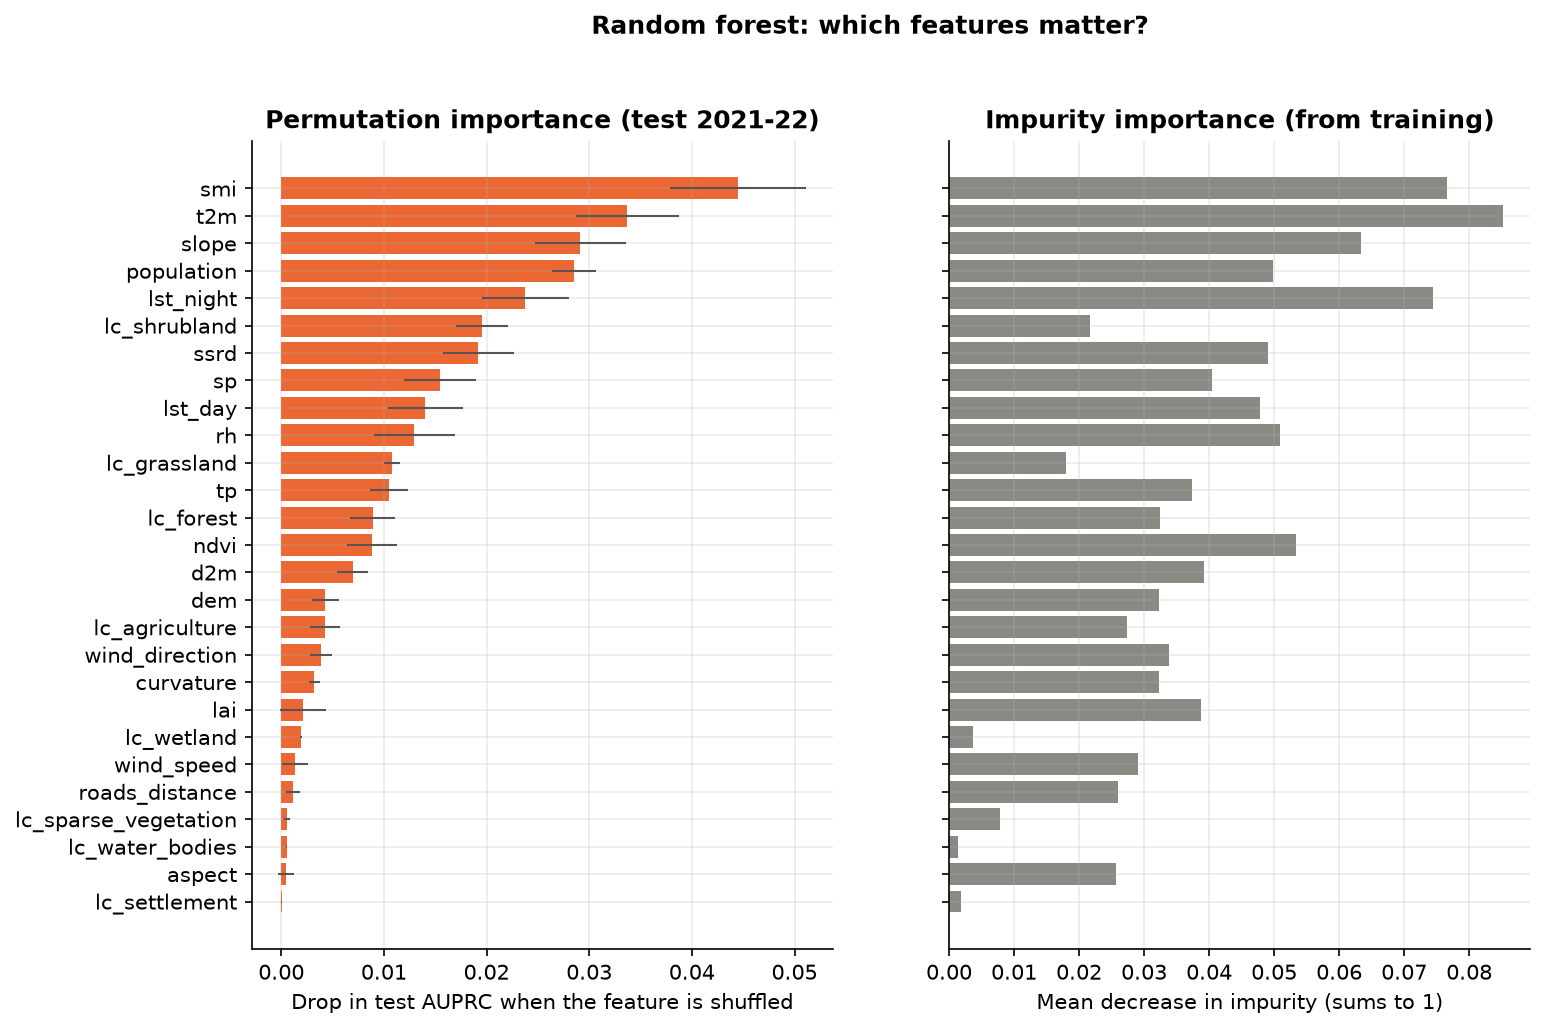
\includegraphics[width=0.85\linewidth]{sophia_rf_feature_importance.png}
    \caption{Random forest feature importance. Left: permutation importance, the drop in test AUPRC (2021--2022) when one feature's values are randomly shuffled; error bars show the spread over 10 shuffles. Right: impurity importance from training, shown for comparison. Soil moisture (smi), air temperature (t2m), slope, population and night-time land-surface temperature (lst\_night) matter most.}
    \label{fig:rf-importance}
\end{figure}

\begin{figure}[H]
    \centering
    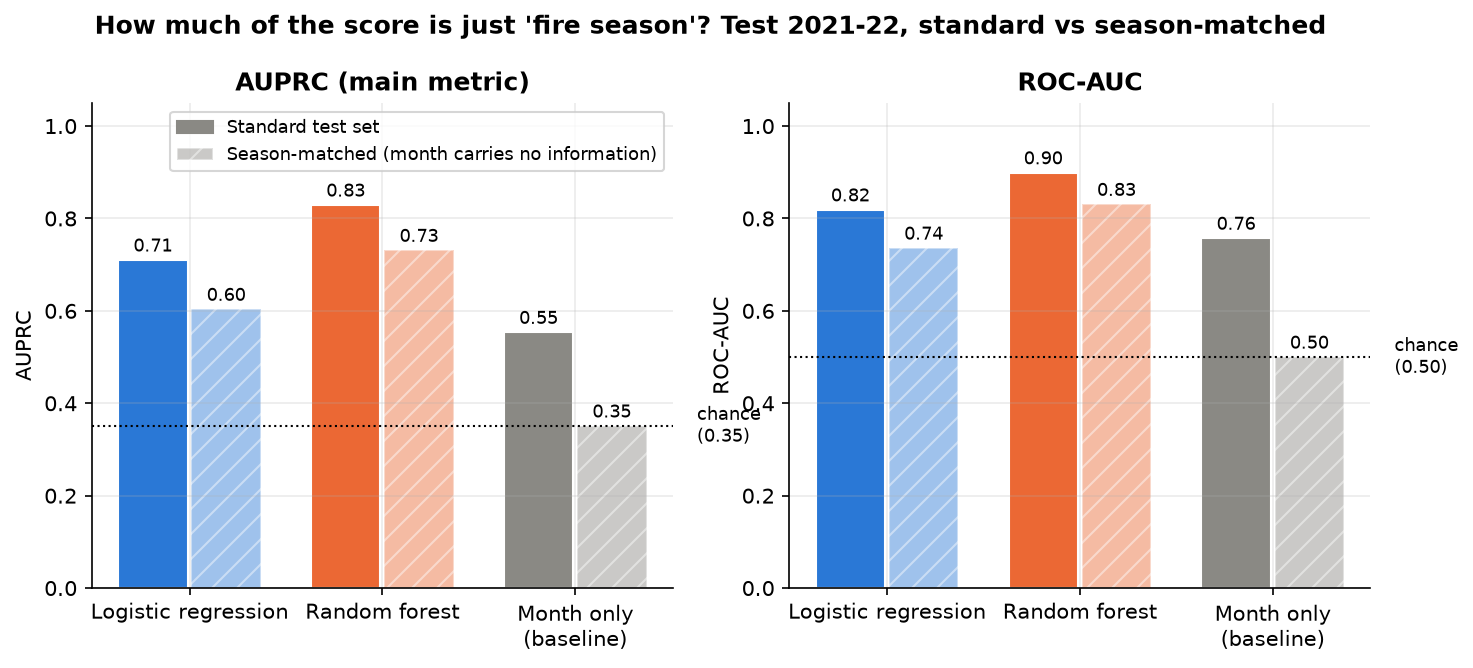
\includegraphics[width=0.85\linewidth]{sophia_season_matched.png}
    \caption{Test scores (2021--2022) of logistic regression, random forest and the month-only baseline, on the standard test set (solid) and season-matched (hatched), where non-fires are reweighted so the month carries no information. The dotted line is random guessing. The month-only baseline falls to chance under season matching, while both models stay well above it.}
    \label{fig:season-matched}
\end{figure}

% ---- Section 5 (comparison) ----
\begin{figure}[H]
    \centering
    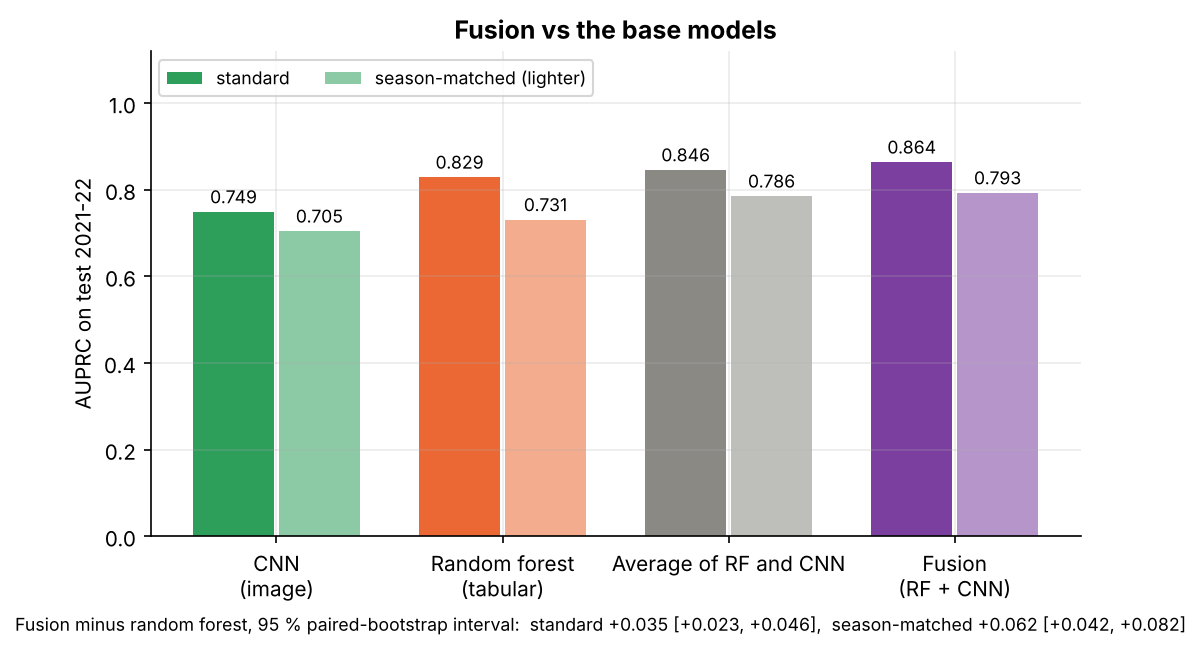
\includegraphics[width=0.85\linewidth]{claudia_fusion_auprc_bars.png}
    \caption{Test AUPRC (2021--2022) of the CNN, the random forest, a plain average of the two, and fusion, on the standard test set (dark) and season-matched (light). Fusion is best in both cases, and its gain over the random forest grows from +0.035 to +0.062 once the season effect is removed; the 95\% paired-bootstrap intervals (bottom) are well above zero.}
    \label{fig:fusion-bars}
\end{figure}

\begin{figure}[H]
    \centering
    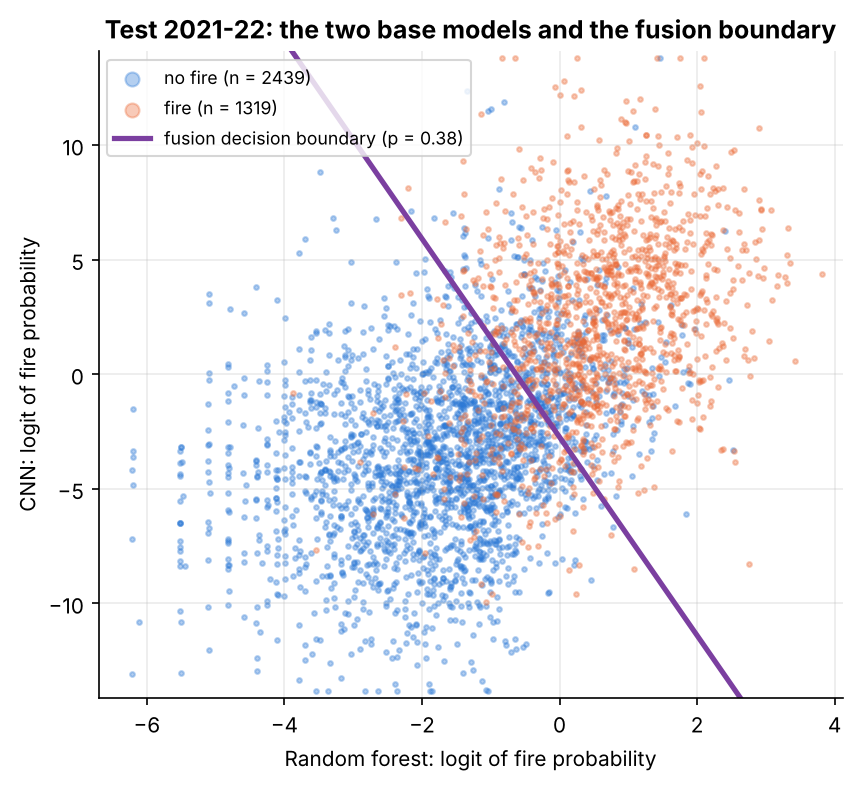
\includegraphics[width=0.7\linewidth]{claudia_fusion_scatter.png}
    \caption{Every test sample (2021--2022) placed by the random forest's prediction (x-axis) and the CNN's prediction (y-axis), both on the logit scale, coloured by the true label. Neither model alone separates fires (orange) from non-fires (blue), but together they do better: the tilted purple line is the fusion decision boundary.}
    \label{fig:fusion-scatter}
\end{figure}
% ---- Sandu: CNN figure (e.g. example tiles or training curve) ----
\begin{figure}[H]
    \centering
    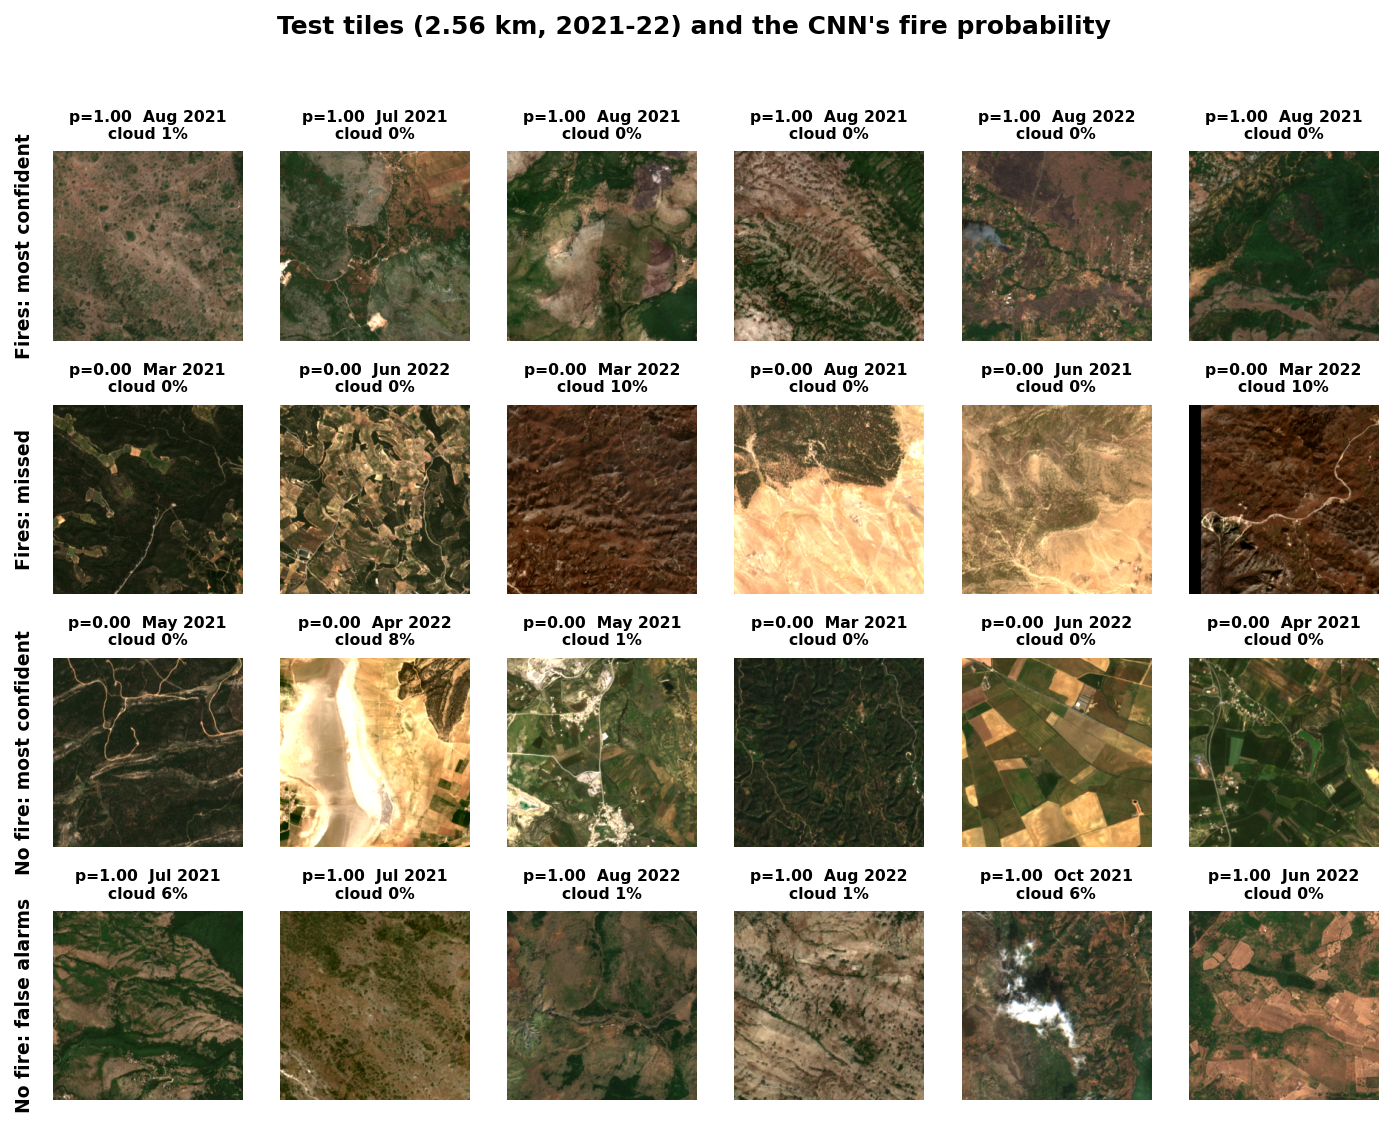
\includegraphics[width=0.85\linewidth]{sandu_example_tiles.png}
    \caption{An example of the Sentinel-2 test tiles from 2021-2022. Each tile captures an area of approximately 2.56\,km and was acquired 1-15 days before the fire day. Above each tile we have put the CNN's fire probability $p$, month of the scene and percentage of cloud coverage. The four rows show fires that the model was most confident about, some of the tiles it missed, where it was confident no fire would happen, and false alarms, where a fire was predicted but did not happen. The model separates dry and sparse land from dense forests, farmlands and water, therefore it recognizes fire prone places and not fire prone days.}
    
    \label{fig:cnn-tiles}
\end{figure}



\begin{figure}[H]
    \centering
    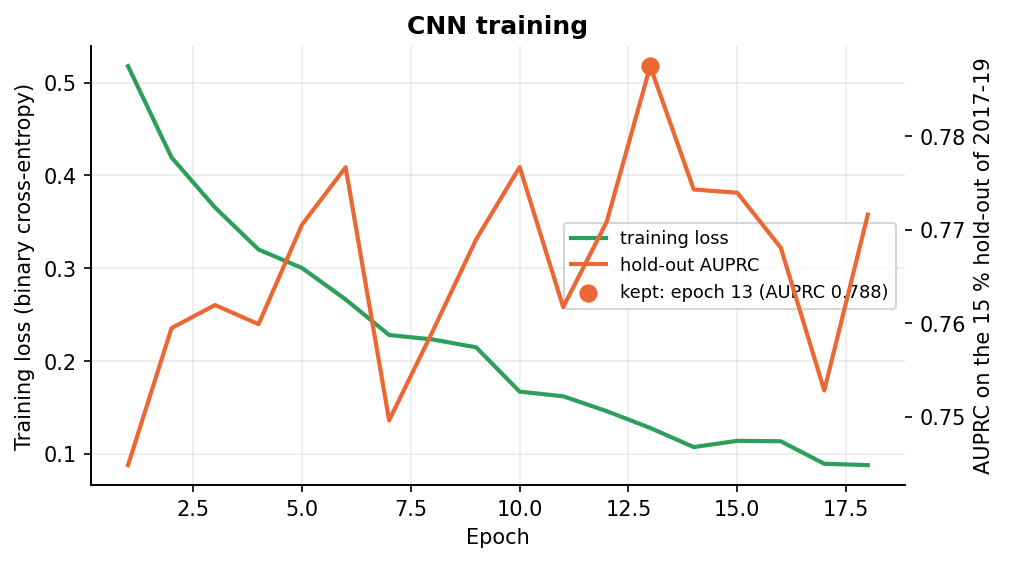
\includegraphics[width=0.75\linewidth]{sandu_training_curve.png}
    \caption{CNN training on 2017--2019: training loss (left axis) and AUPRC on the 15\,\% hold-out (right axis) per epoch. The loss keeps falling to 0.09 whilst the hold-out score flattens out at 0.75--0.79 from epoch 5 and all epochs afterwards, i.e.\ the network might memorise the training tiles without generalising better. Training was stopped after five epochs without improvement; the weights of epoch 13 were kept.}
    \label{fig:cnn-training}
\end{figure}

% ---- Claudia: fusion figure (e.g. fusion weights, or PR curves of all models) ----
% \begin{figure}[H]
%     \centering
%     \includegraphics[width=0.85\linewidth]{claudia_fusion.png}
%     \caption{[Self-contained caption.]}
%     \label{fig:fusion}
% \end{figure}


% ============================================================
% DECLARATION OF CONTRIBUTIONS AND AI USE - everyone
% Required by the brief in every submission.
% ============================================================
\BAMunnumberedsection{Declaration of Contributions and AI Use}
\label{sec:contributions}

\annotation{\textbf{[Rules]} One entry per member: what you did, with concrete outputs. Then one AI-use entry per member for every material use: tool and version, purpose, a representative prompt, what the output was, what you changed or rejected, how you verified it, and which code, figures, sections or decisions it affected. The brief forbids AI-generated prose; say so explicitly for the text.}

\subsection*{Teamwork and Review Process}
We split the work by model (tabular models: Sophia; CNN: Alexandru; fusion: Claudia) and agreed on a shared plan so that all models use the same samples, years and metrics. All code went into a shared GitHub repository through pull requests that another member reviewed and re-ran before merging, and the report was written together in a shared Overleaf project, each member drafting their own sections.

\subsection*{Individual Contributions}

\subsubsection*{Claudia}
Set up the shared repository: the conda environment and package structure, the Mesogeos exploration script, the Track~A downloader and data loader, and the first EDA notebook. Built the fusion branch: the logistic-regression meta-learner on the random forest and CNN probabilities (\texttt{src/forest\_fire\_risk/fusion.py}), its figures, tests, written report (\texttt{reports/fusion/README.md}) and notebook (\texttt{notebooks/fusion.ipynb}), submitted as pull request~\#3. Wrote the Abstract, Section~\ref{sec:recap}, Section~\ref{sec:fusion} and Section~\ref{sec:plan}.

\subsubsection*{Sophia}
Built the tabular branch: the logistic regression and random forest pipeline on the tabular and Sentinel-2 intersection (\texttt{src/forest\_fire\_risk/tabular.py}, side experiments, figures, tests and \texttt{reports/tabular/README.md}), including the year-based cross-validation, the threshold choice, the month-only baseline and the season-matched evaluation, and the predictions used by the fusion model (pull request \#1). Reviewed and re-ran the fusion pull request before approving it. Set up the shared Overleaf project, wrote Section~\ref{sec:tabular} and Section~\ref{sec:comparison}, and added the results table and the tabular and comparison figures.

\subsubsection*{Alexandru}
Built the Sentinel-2 tile pipeline: the Google Earth Engine fetcher, the tile index and image loaders and the pull of 11,579 tiles for 2017 to 2022. Created the map viewer which allowed for easy visualization of dataset for the model. Worked on Track A exploratory analysis notebook and its figures. Worked on the image branch of the model, the ResNet-18 pipeline, figures, test, and written reports as well as the CNN predictions for fusion. Similarly performed the cloud cover analysis that dropped all tiles with above 20\,\% of cloud coverage. Finally, wrote Section ~\ref{sec:cnn} of the report and did the figures referenced, showing error curves and example tiles.


\subsection*{Generative AI and Other Digital Tools}
\textbf{Sophia --- Claude Code (Claude Opus 5.5, Anthropic).} Used for coding the tabular pipeline, clarifying concepts and learning new ones, helping structure the report, checking numbers and references, and trimming wording. I worked iteratively: I described the task, the tool proposed a plan, I reviewed and changed it, and we repeated this until I was satisfied. I checked every output against the code, the result files and the sources, and I am responsible for the final code and text. 

\textbf{Claudia --- Claude Code (Claude Opus 5.5, Anthropic).} Used to understand the repository and the methods (cross-validation, AUPRC, season-matched evaluation, stacking), to write the fusion code, report, figures and notebook, and to structure and edit parts of my report sections. I described each task, reviewed the output, and asked for changes until it matched what I wanted. I verified the fusion results by re-running the pipeline, notebook and tests on my own machine and checking that the numbers matched the result files, and I am responsible for the final code and text.

\textbf{Alexandru --- Claude Code (Claude Fable 5.1, Anthropic).} Used to initially explore the dataset and gain an idea of it. Coded the dataset visualizer on Vercel and used it to help write the code to get the tiles and select the ones used for training. Finally used it to write the code for the actual model and run the training and generate the code for the figures used. I planned out each task asking for feedback and what would be done differently, then reviewed code written by doing an independent run in the command line. I am responsible for the final code and text. 

\end{document}
